\documentclass[prl,aps,twocolumn,showpacs,twocolumngrid,superbib]{revtex4}


\usepackage{graphicx}
\usepackage{amsfonts}
\usepackage{amsmath}
\usepackage{bm}
\usepackage{alltt}
\usepackage{fancyhdr}
\newcommand{\bms}[1]{{\boldsymbol #1}}

%\draft
%\tighten
\pagestyle{fancy}


%\eprint{LA-UR-02-6997}

\begin{document}

\title{
A New View on the Geometry Optimization of Large Molecules            
}

\author{K\'aroly N\'emeth}\email{nemeth@lanl.gov}
\author{Matt Challacombe}

\affiliation{Theoretical Division, Los Alamos National Laboratory, Los Alamos, NM 87545, USA}

\date{\today}

\begin{abstract}
{
This letter peresents a new, efficient alternative to well established
geometry optimization algorithms. The new alternative is based on
fitting gradient surfaces in terms of curvilinear 
internal coordinates and 
determining the roots of the fitted surface. Due to the efficient 
vibrational decoupling of the curvilinear coordinates the 3N-dimesional
optimization problem splits into a quasi non-interacting
set of approximately 3N one-dimensional optimization problems, 
similarly to the self-consistent mean-field concepts of physics.
This allows for robust, linear scaling inmplementation of geometry optimizers.
}

\smallskip
\noindent{\bf Keywords}: 
geometry optimization, linear scaling, 
curvilinear internal coordinates, fitting
\end{abstract}
 
\pacs{?????????????????02.70.-c, 71.15.-m, 71.15.Dx}

\maketitle

\footnotetext[1]{????????????LA-UR-02-6997}

The optimization of molecular structures is one of the most frequent
tasks carried out by computational chemists. 
Structures of large molecules have been optimized so far
only with the use of empirical force-fields, or at most with 
semi-empirical electronic structure theories 
\cite{Stewart_crambin_opt,Schlegel_plasminogen_opt}. However, many important phenomena
can be understood only poorly on these low levels of the theory. 
Such phenomena are e.g. the structural changes of large molecules, 
when beeing put from one solvent into another, the mechanisms of 
enzymatic reactions, the selectivities of ion-channels, etc. 
Geometry optimization is one of the simplest tools to start studying 
these phenomena, since it needs only energy gradients, as input, but 
leads to a welth of relevant structural information.
Not only equilibrium structures, but also transition states and reaction
paths can be determined with the help of efficient optimizers 
\cite{nudged_elastic_band}.

With the advent of linear scaling electronic structure techniques 
\cite{Goedecker99}
energies and gradients are available for large molecules on demanding
levels of the theory. 
However, care must be excercised to reduce the number of energy and 
gradient evaluations during the optimization of molecular structures.
Even though these energies and gradients are available, their 
computational cost is much higher than that of empirical force-fields.
Thus, highly efficient geometry optimizers are needed.

In the last three decades the so-called internal coordinate 
geometry optimizers 
became standard tools of structural optimization when energies 
and forces are calculated by electronic structure theory 
\cite{Pulay_natural_internals}.
Internal coordinates describe the internal motions of molecules 
by displacements of chemical entities, such as bond-stretches, 
valence angle bendings and torsions of dihedral angles. These 
coordinates are curvilinear, since they can be composed
as non-linear functions of the Cartesian coordinates of atomic nuclei.

An important property of these chemical
internal coordinates
is that they significantly reduce the harmonic and higher order 
vibrational coupling, as compared to Cartesian coordinates. 
In internal coordinate representation it is much easier to estimate 
harmonic and higher order force-constants than in Cartesian. Even
if accurate harmonic force-constants are available, internal coordinates
are superior for geometry optimization, since anharmonic effects are
usually large. In practice, accurate harmonic force constants are 
not available for geometry optimization, since their calculation 
is very expensive.

Internal coordinates represent a natural energy and 
length-scale separation of molecular movements.
The stiffest molecular motions are usually those of strechings, while 
the softest ones are related to torsions. This letter internal 
coordinates are almost exclusively responsible for the large 
conformational motions of proteins and molecular aggregates.
Typical harmonic force constants for stretches are in the order of 
0.5 atomic units (a.u.), those of bendings are of 0.2 a.u. and the
torsions are around 0.1 a.u or below. 
These typical values however, can vary a lot.
For example, a double bond is much stiffer than a single bond or 
a hydrogen-bridge. Also, the values of the force constants depend
on the actual conformation of the molecule. Thus, a rough estimate
of these force constants is usually not satisfactory 
for an effective optimization
of complex molecules. However it is often enough in the case of small
molecules \cite{fogarasi_diaghess}.

In order to get more accurate curvature information about the 
potential energy surface the so-called Hessian-matrix update schemes
are used \cite{RFletcher}. 
Hessian matrix update schemes are derived from the assumption of a 
harmonic potential energy surface. A series of rank-1 updates
can build the exact Hessian matrix using gradients and displacements
of consequtive geometry optimization steps.
E.g. for a 100 atom system, on an ideal harmonic surface 300 rank-1
updates are necessary to to build the exact Hessian. The success
of Hessian update schemes is based on, that for geometry optimization
an imperfect Hessian is enough to bring the molecule to a local 
optimum by quasi-Newton steps. In order to maintain convergence 
to a local
minimum instead of a transition state, the positive definite nature
of the updated Hessian must always be ensured. However, as 
an approximate Hessian cannot provide absolute certainty about the 
nature of a local extremum, the exact Hessian remains the only tool
to examine the quality of the extremum with full reliability. 
A numerical study of the qulity of the extremum has been provoded
in Ref \cite{Wales_saddlepoint} for the case of 
gradients-only optimizations.

The updated Hessian matrices require ${\cal{O}}(N^{2})$ storage, thus
their use becomes a computational bottleneck for large molecules.
There are a few approaches to overcome this limitation.
The most widely used one is the Limited Memory BFGS (LBFGS) 
technique of Nocedal
e.al. \cite{nocedal_lbgs}. This technique does never explicitely 
construct the full Hessian matrix. Istead, it carries out all 
the necessary operations by an implicite application of the Hessian
via its component vectors. LBFGS
has the limitation that it can use only a small number of remembered
steps.
LBFGS has never been used in conjuction with internal coordinates
for large systems yet.
Another useful approach has been constructed very recently by Bofill,
Anglada et.al. \cite{bofill_lanczos}. This approach is similar
to LBFGS in the sense that it avoids the use of the explicite
Hessian, but it can calculate necessary eigenvectors of the 
Hessian by a Lanczos-type algorithm. A
similar approach is the ${\cal{O}}(N^{2})$ scaling iterative
scheme of Schlegel and Farkas \cite{schlegel_on2iter}.
In Stewart's approach, an update
formula of the inverse Hessian has been used, and the full explicite
Hessian has been truncated by spacial thresholding and stored in a 
sparse matrix fashion \cite{Stewart_crambin_opt}. 
The reported performance
of Stuart's scheme was rather poor on large molecules.

The efficient use of internal coordinates for large molecules has 
been limited by another important factor. That is the coordinate
transformation problem, which must be carried out very frequently
to transform Cartesian vectors and curvilinear internal ones into each
other. This problem has found a linear scaling solution   
only in very recent developments. 
\cite{paizs_coordtrf1,nemeth_coordtrf1,paizs_coordtrf2,nemeth_coordtrf2,billeter_coordtrf,andzelm_coordtrf,kudin_coordtrf}. 

In the present letter we introduce a fundamentally new approach
to molecular geometry optimization. We call this approach the
Fitting of Internal Coordinate Gradients
(FICG) technique. This new approach is very simple
to implement, scales fully linearly with system size 
and is very efficient for both small and large molecules.

The new algorithm is based on an assumption widely used in molecular 
modelling. Namely, that
the potential energy function of a molecule can be decomposed to a sum
of univariate functions, each of them depending only on a   
chemical curvilinear coordinate, such as bond, bond angle
or torsional angle: 
\begin{equation}
V(\bms{X}) = \sum_{n} V_{n}(\bms{r}_{n}) ,
\end{equation}
where $V$ represents the potential energy, $\bms{X}$ the nuclear
coordinates, and $\bms{r}_{n}$ the $n$-th internal coordinate.
This assumption is, again, based on the
experience, that harmonic and higher order force constants are
effectively decoupled in internal coordinate representation.

Finding the equilibrium of the molecular
structure is equivalent to the minimization of the forces along internal
coordinates. Of course, in a real situation there is coupling
between the internal coordinates, and therefore the gradients over
internal coordinates are functions of the molecular environment as well:
\begin{equation}
\bms{g}_{k}^{(i)} = \bms{g}_{k}^{(i)}\left( \bms{r}_{k}^{(i)},\bms{R}_{k}^{(i)} \right) .
\end{equation}
Here, $g_{k}^{(i)}$ is the gradient acting 
on the $k$-th internal coordinate
at the $i$-th step of the optimization process, $r_{k}^{(i)}$ is 
the value of the internal coordinate and $R_{k}^{(i)}$ is the position
of the rest of the molecule. 

The energy gradients must show progression during the optimization.
They must tend to zero. 
Indeed, they show stronger or weaker tendencies.
See eg. Fig. \ref{NH3outp6} for a typical progression of gradients 
during geometry optimization.
\begin{figure}[h]
\resizebox*{3.5in}{!}{\includegraphics{1_6_6_Data.eps}}
\caption{
\small  
Progression of gradients on a valence angle bending coordinate of
ammonia. The optimization was started from near planar geometry, i.e.
from the vicinity of a transition state, and converged to a local 
minimum of the potential energy surface. The numbers in the picture
indicate the sequence of optimization steps.
\label{NH3outp6}
}
\end{figure}

These tendencies can be revealed by
fitting curves along the gradient vs coordinate data pairs
of internal coordinates, based on the data of the few most
recent optimization steps.
A similar fitting procedure has been applied to
the parametrization of empirical
force-fields \cite{force-field-fitting}. 
In geometry optimization, the fitting process
must be done at each step, to refresh or enrich the information
held by these curves. 
The roots of the fitted curve can easily be determined, 
and they provide a new guess for the coordinate value, where the
gradient is expected to vanish.
By repeating the curve fitting, and setting the values of internal
coordinates to the predicted roots of the curves,
the structure of the molecule
converges. The convergence is a self-consistent procedure, since
it smoothes out the the coupling effects on the fitted curves, and thus
it makes predictions more and more accurate.

The fitting of curves happens through 
well established and robust algorithms, which are available in standard 
computational libraries 
\cite{slatec}. 
It is important, to note,
that data points are weighted before the fit. The weights, 
$w_{k}^{(i)}$, are
measures of the stuctural tension in the vicinity of the $k$-th internal
coordinate at the $i$-th geometry. They account for the effect of the 
environment $R_{k}^{(i)}$ on the $k$-th internal coordinate. 
The weights are computed as
\begin{equation}
w_{k}^{(i)} = \left[ \sum_{l} g_{l}^{(i)} \frac{1}{|H_{ll}^{}|} g_{l}^{(i)} \right]^{-1} ,
\end{equation}
where $l$ indicates the internal coordinates which have atoms in common
with the $k$-th internal coordinate, i.e. which are in the spacial 
vicinity of the $k$-th coordinate. $H_{ll}^{}$ is an estimate
of the diagonal matrix element of the Hessian for the $l$-th 
internal coordinate. $H_{ll}^{i}$ is calculated as the local tangent
of the gradient curve of a primary fit. 
%\begin{equation}
%H_{ll}^{i} = \left . \frac{\partial g_{l}^{(i)}}{\partial r_{l}^{}} \right|_{r_{l}^{}=r_{l}^{(i)}}
%\end{equation}
The primary fit is done with 
the weights $w{'}_{k}^{(i)} = 1/g_{k}^{(i)2}$ usual to 
estimate relative errors.
The weights $w_{k}^{(i)}$ correspond to inverse energy changes
and they increase when the tension in a given 
local environment decreases. They provide
a simple way to observe coupling between neighbouring internal
coordinates.

The statistical F test is used, to decide about the order of the fit. 
So far no higher than quadratic fit has been considered.

If the gradient curve has a negative tangent at the position
of the root, it is an indication for a transition state. 
Eg. in Fig. \ref{NH3outp6}
the tangent of the gradient curve is negative 
in the vicinity of the planar
structure (structure \#1). This should be so, since the planar
ammonia represents a transition state. The tangent of the gradient 
curve thus offers a
convenient tool to control convergence to minima or transition state.
We plan to elaborate a transition state finding tool based on this 
principle. However, in the present letter we restrict the discussion
to the localization of minima. Whenever the local tangent  
of the gradient curve
is negative, the optimizer moves the actual geometry away from 
the transition state.
%Internal coordinates are redefined at each step of the optimization.
%This is important for large molecules, since conformational
%changes may lead to the appearence of new bonds, eg. hydrogen bridges,
%while some other bonds may disappear.
%for the large paper, note, that merging of topologies is 
%necessary at this point for the sake of stable coordinate 
%transformations.

It is typical in one-dimensional root-finding, to bracket the root of
the function. After the root is bracketed, usual techniques, like
the golden section can be applied. In the case of geometry optimization
we have to find the root of a varying function, since the form of
the gradient curve converges only at the end the optimization.
For this we want to bracket the root at each step, instead of
going directly for it. For the purpose of bracketing the standard 
uncertainty, $\sigma$ of the predicted root is determined. 
Then, an extra amount of displacement, proportional to $\sigma$
is used to overshoot the predicted root.

%The optimizer has been  
%implemented such that it tries to bracket the 
%root, $x_{k0}^{(i)}$ of the gradient curve, 
%instead of going directly for it.  
%Bracketing is a typical technique applied in one-dimensional 
%root-finding. For the bracketing, we use the covariance matrix of the 
%fitted parameters, to determine $\sigma_{k}^{i}$, 
%the uncertainty of the predicted root $x_{k0}^{(i)}$. Then, 
%the value of the given internal coordinate is set to $x_{k}^{(i+1)}$:
%\begin{equation}
%x_{k}^{(i+1)} = x_{k0}^{(i)} + \sigma*sign(x_{k0}^{(i)}-x_{k}^{(i)})  ,
%\end{equation}
%with $x_{k}^{(i)}$ representing the value of the 
%internal coordinate in the most recent $i$-th step of the optimization.

We will provide detailed information about the technology of 
the Fitting of Internal Coordinate Gradients
optimizer in a forthcoming paper \cite{bisect-paper}.

The performance of this initial implementation of the FICG optimizer
has been tested on a 
series of small molecules, called Baker's test set \cite{bakerstest}.
Table \ref{Bakers_test} lists all the test results
in order to convince
the reader, that our fundamentally new approach to geometry optimization
works as well on small molecules as the best traditional techniques.
\begin{table}[h]
\caption{
Geometry optimization steps of small molecules (upto 30 atoms)
of the Baker's test set. Calculations have been carried out 
with the Hartree-Fock model in STO-3G basis set.
At convergence, Cartesian force vectors were shorter 
than $3\times10^{-4}$ atomic units, on all atoms. Energies have been
reproduced to all digits to given values in Ref. \cite{bakerstest}.
Note, that all calculations of this table used standard primitive 
internal coordinates, except the one by Bakken \cite{bakken}, 
which was based on the so called extra redundant coordinates.
}
\label{Bakers_test}
\squeezetable
\begin{tabular}{lccccc}
\toprule
Molecule               & Present  & Bakken & Eckert  & Lindh &  Baker  \\
         & work & {\it{et al.}} & {\it{et al.}} & {\it{et al.}} &    \\
         &(FICG) &  \cite{bakken} &  \cite{eckert} & \cite{lindh} &  \cite{bakerstest} \\
\colrule
Water                  &   4    &   4    &    4    &    4   &   6     \\
Ammonia                &   4    &   5    &    6    &    5   &   6     \\
Ethane                 &   4    &   3    &    4    &    4   &   5     \\
Acetylene              &   4    &   4    &    6    &    5   &   6     \\
Allene                 &   3    &   4    &    4    &    5   &   5     \\
Hydroxysulphane        &   7    &   7    &    7    &    8   &   8     \\
Benzene                &   2    &   3    &    3    &    3   &   4     \\
Methylam.              &   4    &   4    &    5    &    5   &   6     \\
Ethanol                &   5    &   4    &    5    &    5   &   6     \\
Acetone                &   5    &   4    &    5    &    5   &   6     \\
Disilyl ether          &   9    &   8    &    9    &   11   &   8     \\
1,3,5-trisilacycl.     &   6    &   9    &    6    &    8   &   8     \\
Benzaldehyde           &   4    &   4    &    5    &    5   &   6     \\
1,3-difluorobenz.      &   4    &   4    &    5    &    5   &   5     \\
1,3,5-trifluorob.      &   3    &   4    &    4    &    4   &   5     \\
Neopentane             &   5    &   4    &    4    &    5   &   5     \\
Furan                  &   6    &   5    &    6    &    7   &   8     \\
Naphtalene             &   6    &   5    &    6    &    6   &   5     \\
1,5-difluoronapht.     &   6    &   5    &    6    &    6   &   6     \\
2-hydroxibicyclop.     &   7    &   9    &    9    &   10   &  15     \\
ACHTAR10               &  11    &   8    &    9    &    8   &  12     \\
ACANIL01               &  11    &   7    &    8    &    8   &   8     \\
Benzidine              &   9    &   9    &    7    &   10   &   9     \\
Pterin                 &  12    &   8    &    9    &    9   &  10     \\
Difuropirazine         &   7    &   6    &    7    &    7   &   9     \\
Mesityl oxide          &   5    &   5    &    6    &    6   &   7     \\
Histidine              &  10    &  16    &   14    &   20   &  19     \\
Dimethylpenthane       &   7    &   9    &   10    &   10   &  12     \\
Caffeine               &   6    &   6    &    7    &    7   &  12     \\
Menthone               &  17    &  12    &   10    &   14   &  13     \\
\colrule
Total                  & 193    & 185    &  196    &  215   & 240     \\
\botrule
\end{tabular}
\end{table}
While retaining the same efficiency for small molecules, our technique
is fully linear scaling as opposed to any other internal 
coordinate optimizers reported so far. In addition, it is far simpler
to implement then any traditional alternatives.
This allowes the fast and efficient 
extension of geometry optimization 
to large molecules, where scaling issues are important.
In order to illustrate the performance of our optimizer on large
molecules, we show the convergence of the molecular total energy
during the course of the optimization of a 257 atom
fragment of Protein Kinase A, in Figs. \ref{logn-logde} 
and \ref{order-of-conv}. 10 periferial atoms have been 
constrained, in order to mimic the rest of the enzyme, 
the rest of the molecule was allowed to move freely.
The optimizations have been carried out 
using MondoSCF \cite{MondoSCF}, a linear scaling electronic structure
program system, in the PBE density functional model and 
STO-2G basis set, with 0.1 milliHartree resolution of the energies.
The convergence was smooth with minor jumps in the energy.
A first order convergence is typical for the bulk of the optimization
of larger molecules. For smaller molecules, like the ones of Baker's
test set, the order of convergence is between linear and quadratic,
with an acceleration towards convergence.
\begin{figure}[h]
\resizebox*{3.5in}{!}{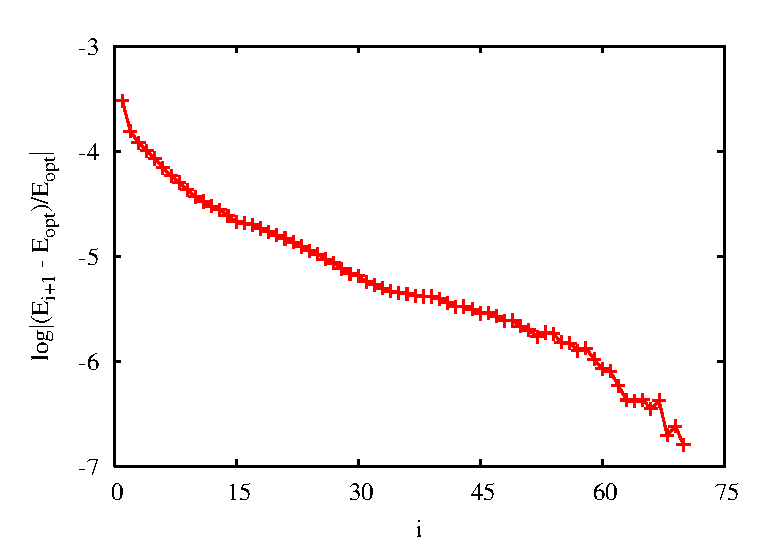
\includegraphics{curve3.eps}}
\caption{
\small  
The error of the energy has an exponential decline during
the optimization of a 257 atom protein kinase A fragment. 
$i$ denotes the serial number of steps,
$E_{opt}$ is the optimum energy.
\label{logn-logde}
}
\end{figure}


\begin{figure}[h]
\resizebox*{3.5in}{!}{\includegraphics{curve2.eps}}
\caption{
\small  
Relative errors of the energy show linear improvement.
Thus, the convergence is of first order. Higher order
convergence can be expected only beyond the milliHartree
energy resolution for this molecular size.
\label{order-of-conv}
}
\end{figure}

In this letter we have presented a fundamentally new approach
to the optimization of molecular structures.
We have shown, that internal coordinates representing chemical 
entities can efficiently be optimized, without
ever accounting for explicite vibrational couplings, as traditional
optimization techniques do. This allowes an efficient
extention of quantum-level modeling to geometrical processes
of biomolecules, such as enzymatic reactions, macroscopic quantum 
effects in ion-channels or solvent effect on biomolecules.
Our technique can also be used
to provide simple and accurate updates of force-fields
for molecular dynamics simulations, based on the availability of
quantum-mechanical forces.

\bibliography{mondo_new}







\end{document}
